Various technologies are needed for detecting devices on the network. In this chapter, four technologies are explained: MIB, SNMP, LLDP, and NETCONF.

Management Information Base (MIB) describes a data structure and is used in different technologies like SNMP. The data is structured hierarchically in a tree. A saved object can be addressed via a sequence of numbers or an ASCII string sequence. It is using Formal Abstract Syntax Notation One (ASN.1) to describe the database and its entries.

Simple Network Management Protocol (SNMP) is a network monitoring and management protocol, developed in 1988 by the
Internet Engineering Task Force (IETF). Over the years, multiple versions of SNMP have been released, but only three
of them are mainly used: v1, v2c, and v3. The communication between network devices is handled by agents. There is one master agent, called AgentX, which communicates with other master agents. SNMP supports multiple instructions for getting and setting data from the devices.

Link Layer Discovery Protocol (LLDP) is an open and vendor-independent Layer 2 Protocol. Its purpose is
to advertise the identity and capabilities to the connected network neighbors. Each device runs an agent, which collects the data sent by other devices. Because LLDP is a Layer 2 Protocol, it does not need an IP address to transmit its information.

Network Configuration Protocol (NETCONF) is a network monitoring and management protocol, published in 2006 as a successor of SNMP. It exchanges data encoded with XML with remote procedure calls. The advantages over SNMP are a modern, secure , and session-based communication, detection of capabilities, and the modern data description language YANG.


\section{MIB - Management Information Base}
\label{Section:MIB}

The Management Information Base (MIB) is used to describe network entities. It was created to monitor, manage, and control network entities over a remote management protocol. It was first defined in RFC 1155\cite{RFC:RFC1155:1990}, RFC 1156\cite{RFC:RFC1156:1990} and RFC 1157\cite{RFC:RFC1157:1990} by IEFT. Its main purpose was to provide a standardized Data Modeling Language for SNMP (Section \ref{Section:SNMP}), but it can also be used for other remote management protocols. The current valid standards for MIB are RFC 1155\cite{RFC:RFC1155:1990} and RFC 1235 \cite{RFC:RFC1213:1991}.

The MIB represents a hierarchical database, that is a tree. The root node of the tree is a MIB called MIB-I \cite{RFC:RFC1155:1990}, which can be extended by submodules defined in other MIBs. Elements in the tree are called \textit{managed objects} and have a unique id on their level, which is called Object Identifier (OID). With the OID it is possible to address one specific object in the tree, by describing the path from the root object to the object itself. The OID can be expressed as a sequence of numbers (.1.3.6.1.4.1) or as an ASCII string sequence (.iso.org.dod.internet.private.enterprise), however, they can also be mixed (.iso.org.dod.1.4.1). A simplified graphical representation of such a MIB tree structure can be found in Figure \ref{Figure:MIB-MIBTree}.

MIBs are using Formal Abstract Syntax Notation One (ASN.1)\cite{ISO:ISO8824-1:2015} as a formal description language and are normally saved in text files with the file extension .mib. Other MIBs can be imported into one MIB and their definitions and types can be reused. MIBs are normally defined and maintained by IEFT and IEEE, but also by hardware and software vendors. There are multiple sources to acquire the MIBs, they can be found in RFC documents, on websites from vendors, as well as on general websites like \url{http://mibdepot.com}.


\begin{figure}[!ht]
\centering
\begin{tikzpicture}
    \tikzstyle{object}      = [shape=rectangle, draw, align=center]
    \tikzstyle{relation}    = [draw,-]
    \tikzstyle{relation_red}= [draw,thick,red,-]

    \node (OID) {};

    \node [object, below=of OID]    (OID1) {ISO\\1};
    \node [object, left=of OID1]    (OID0) {CITT\\0};
    \node [object, right=of OID1]   (OID2) {ISO - CCIT\\2};
    \node [object, right=of OID2]   (OID3) {...\\3};

    \node [object, below=of OID1]   (OID1_2) {member body\\2};
    \node [object, left=of OID1_2]  (OID1_1) {..\\1};
    \node [object, right=of OID1_2] (OID1_3) {org\\3};
    \node [object, right=of OID1_3] (OID1_4) {...\\4};

    \node [object, below=of OID1_3]     (OID1_3_6) {DoD\\6};
    \node [object, left=of OID1_3_6]    (OID1_3_5) {...\\5};
    \node [object, right=of OID1_3_6]   (OID1_3_7) {...\\7};

    \node [object, below=of OID1_3_6]   (OID1_3_6_1) {Internet\\1};
    \node [object, left=of OID1_3_6_1]  (OID1_3_6_0) {...\\0};
    \node [object, right=of OID1_3_6_1] (OID1_3_6_2) {...\\2};

    \node [object, below=of OID1_3_6_1]     (OID1_3_6_1_4)    {private\\4};
    \node [object, left=of OID1_3_6_1_4]    (OID1_3_6_1_3)    {experimental\\3};
    \node [object, left=of OID1_3_6_1_3]    (OID1_3_6_1_2)    {management\\2};
    \node [object, left=of OID1_3_6_1_2]    (OID1_3_6_1_1)    {...\\1};
    \node [object, right=of OID1_3_6_1_4]   (OID1_3_6_1_5)    {...\\5};

    \node [object, below=of OID1_3_6_1_4]   (OID1_3_6_1_4_1) {enterprises\\1};
    \node [object, left=of OID1_3_6_1_4_1]  (OID1_3_6_1_4_0) {...\\0};
    \node [object, right=of OID1_3_6_1_4_1] (OID1_3_6_1_4_2) {...\\2};

    \node [object, below=of OID1_3_6_1_2]   (OID1_3_6_1_2_1) {MIB-2\\1};
    \node [object, left=of OID1_3_6_1_2_1]  (OID1_3_6_1_2_0) {...\\0};
    \node [object, right=of OID1_3_6_1_2_1] (OID1_3_6_1_2_2) {..\\2};


    \path [relation]    (OID.south) -- (OID0.north);
    \path [relation_red](OID.south) -- (OID1.north);
    \path [relation]    (OID.south) -- (OID2.north);
    \path [relation]    (OID.south) -- (OID3.north);

    \path [relation]    (OID1.south) -- (OID1_1.north);
    \path [relation]    (OID1.south) -- (OID1_2.north);
    \path [relation_red](OID1.south) -- (OID1_3.north);
    \path [relation]    (OID1.south) -- (OID1_4.north);

    \path [relation]    (OID1_3.south) -- (OID1_3_5.north);
    \path [relation_red](OID1_3.south) -- (OID1_3_6.north);
    \path [relation]    (OID1_3.south) -- (OID1_3_7.north);

    \path [relation]    (OID1_3_6.south) -- (OID1_3_6_0.north);
    \path [relation_red](OID1_3_6.south) -- (OID1_3_6_1.north);
    \path [relation]    (OID1_3_6.south) -- (OID1_3_6_2.north);

    \path [relation]    (OID1_3_6_1.south) -- (OID1_3_6_1_1.north);
    \path [relation]    (OID1_3_6_1.south) -- (OID1_3_6_1_2.north);
    \path [relation]    (OID1_3_6_1.south) -- (OID1_3_6_1_3.north);
    \path [relation_red](OID1_3_6_1.south) -- (OID1_3_6_1_4.north);
    \path [relation]    (OID1_3_6_1.south) -- (OID1_3_6_1_5.north);

    \path [relation]    (OID1_3_6_1_2.south) -- (OID1_3_6_1_2_0.north);
    \path [relation]    (OID1_3_6_1_2.south) -- (OID1_3_6_1_2_1.north);
    \path [relation]    (OID1_3_6_1_2.south) -- (OID1_3_6_1_2_2.north);

    \path [relation]    (OID1_3_6_1_4.south) -- (OID1_3_6_1_4_0.north);
    \path [relation_red](OID1_3_6_1_4.south) -- (OID1_3_6_1_4_1.north);
    \path [relation]    (OID1_3_6_1_4.south) -- (OID1_3_6_1_4_2.north);

\end{tikzpicture}
\caption{Shows a simplified MIB-Tree, where red marks the path for .1.3.6.1.4.1 or .iso.org.dod.internet.private.enterprise (Adaption based on \cite{Mueller:MIBTree:2006})}
\label{Figure:MIB-MIBTree}
\end{figure}

\subsection{Names}
\label{Section:MIB-Names}

A \textit{name} is used to uniquely identify an object, regardless of the semantic association (standard document, network device, etc.), this concept is called Object Identifier (OID). An OID is a sequence of integers traversing a global tree. The root of the tree is connected to a number of labeled nodes via edges. Each node may have labeled children, also called a subtree. This concept may be repeated arbitrarily. A label is defined as a pairing of a brief textual description and an integer number. The root node itself is unlabeled and has at least three children (see Figure \ref{Figure:MIB-MIBTree}). These children are defined in \cite{RFC:RFC1155:1990} and may be extended by other standards. The three main nodes are:

\begin{minipage}{\textwidth}
\begin{itemize}
    \item ccitt(0) by the International Telegraph and Telephone Consultative Committee
    \item iso(1) by the International Organization of Standardization
    \item joint-iso-ccitt(2) by ISO and CCITT
\end{itemize}
\end{minipage}


The iso(1) node has a designated child node with the name org(3), that can be used by other international organizations. These organizations have their own subtrees below their child task. Two subtrees got assigned to the U.S National Institutes of Standard and Technology and one of them has been transferred to the U.S. Department of Defense, dod(6). The Department of Defense has allocated a node to the \textit{internet} community, to be managed by the Internet Activities Board (IAB). The definition of the \textit{internet} can be seen in Listing \ref{Listing:MIB-InternetNode}. The \textit{internet} object can be identified as 1.3.6.1 or as .iso.org.dod.internet. The IAB also defined four subnodes of internet(1), this can be seen in Listing \ref{Listing:MIB-InternetSubNodes}.

\begin{lstlisting}[label=Listing:MIB-InternetNode,captionpos=b,caption={Definition of a node, internet node used as an example (from \cite{RFC:RFC1155:1990})}]
    internet   OBJECT IDENTIFIER ::= { iso org(3) dod(6) 1 }
\end{lstlisting}

\begin{lstlisting}[label=Listing:MIB-InternetSubNodes,captionpos=b,caption={Definition of subnodes, internet subnodes used as an example (from \cite{RFC:RFC1155:1990})}]
    directory     OBJECT IDENTIFIER ::= { internet 1 }
    mgmt          OBJECT IDENTIFIER ::= { internet 2 }
    experimental  OBJECT IDENTIFIER ::= { internet 3 }
    private       OBJECT IDENTIFIER ::= { internet 4 }
\end{lstlisting}


The directory(1) subtree has not been defined in \cite{RFC:RFC1155:1990}, but it discusses how OSI Directory may be used on the Internet. OSI Directory is also known as X.500 and is a system to lookup named objects. 

The mgmt(2) subtree is used for IAB-approved documents. The subnode mgmt(1) is used for newer approved versions of the Internet standard Management Information Base, defined by RFC.

The experimental(3) subtree is used for Internet experiments and is managed by the Internet Assigned Numbers Authority of
the Internet. They may define requirements on how this tree has to be used.

The private(4) subtree is used to define unilateral objects. It is managed by the Internet Assigned Numbers Authority(IANA) of the Internet. It has an enterprise(1) subtree, which can be used by companies to define their subtrees. To add a subtree in this subtree, an enterprise identification number needs to be registered.

\subsection{Syntax}
\label{Section:MIB-Syntax}

The structure of objects is described using the ASN.1 syntax, but the full generality of ASN.1 is not permitted. For primitives, only the following ASN.1 primitives are allowed: integer, octet string, the object identifier, and null. If an enumerated integer is used, there shall be no element with value 0.

Multiple non-primitive types can be used. The ASN.1 constructor sequence can be used to generate lists and tables. New types can be defined, but remain ASN.1 primitive types, lists, tables and, other application types. Other application types are:

\begin{minipage}{\textwidth}
\begin{itemize}
    \item \textbf{NetworkAddress:} This choice type represents an address from one of several internet protocol families.
    \item \textbf{IpAddress:} This type represents an internet address, represented as an octet string in network-byte order.
    \item \textbf{Counter:} This represents a non-negative integer value that can be increased. It wraps around if the maximum value is reached and starts incrementing from zero again.
    \item \textbf{Gauge:} This represents a non-negative integer value that can be increased and decreased, but latches at the minimum and maximum value.
    \item \textbf{TimeTicks:} This represents a non-negative integer value, that is getting incremented every hundredth of a second since an epoch. The epoch needs to be defined and explained in the description of this type.
    \item \textbf{Opaque:} This represents data with special encoding. Details can be found in RFC 1155 (\cite{RFC:RFC1155:1990}).
\end{itemize}
\end{minipage}


\subsection{Objects}
\label{Section:MIB-Managed_Objects}

Objects must be defined in a MIB. A MIB can contain a collection of object definitions. An object may refer to another object defined in the same or another MIB. The MIB defines the following items for each object:

\begin{minipage}{\textwidth}
\begin{itemize}
    \item \textbf{Name:} Consists of a textual name and Sub-OID, and is also known as an object descriptor. It's not allowed to use 0 as a Sub-OID.
    \item \textbf{Syntax:} Defines the type of the object (see Section \ref{Section:MIB-Syntax}).
    \item \textbf{Definition:} Describes the usage of the object.
    \item \textbf{Access:} Defines the access rights of the object. Access permissions can be one of: "read-only", "read-write", "write-only", "not-accessible".
    \item \textbf{Status:} The object can be classified as "mandatory", "optional" or "obsolete".
\end{itemize}
\end{minipage}


A management protocol that is using MIBs must provide a way to access a simple non-aggregate object. The management protocol needs to define if an aggregate object can be accessed. If an object refers to multiple instances, it also needs to specify which instance of an object has been returned. An example of an object definition can be seen in Listing \ref{Listing:MIB-Object}.

\begin{lstlisting}[label=Listing:MIB-Object,captionpos=b,caption={Example of an object definition (taken from \cite{RFC:RFC1155:1990})}]
    OBJECT:
    -------
        atIndex { atEntry 1 }
    
    Syntax:
        INTEGER
    
    Definition:
        The interface number for the physical address.
    
    Access:
        read-write.
    
    Status:
        mandatory.
\end{lstlisting}

\newpage
\subsection{Versions}
\label{Section:MIB-Versions}

Every MIB document makes the previous version of the same document obsolete. It is forbidden to change the OID of an object between versions of a MIB document. The standard RFC1155 (see \cite{RFC:RFC1155:1990}) defines rules to remain constant regarding semantics and simplify implementing support for multiple versions of a MIB \cite{RFC:RFC1155:1990}:

''New versions may:

\begin{minipage}{\textwidth}
\begin{itemize}
    \item declare old object types obsolete (if necessary), but not delete their names;
    \item augment the definition of an object type corresponding to a list by appending non-aggregate object types to the object types in the list; or,
    \item define entirely new object types.
\end{itemize}
\end{minipage}


New versions may not:

\begin{minipage}{\textwidth}
\begin{itemize}
    \item change the semantics of any previously defined object without
    changing the name of that object.''\cite{RFC:RFC1155:1990}
\end{itemize}
\end{minipage}


\subsection{MIB Files}
\label{Section:MIB-MIB_Files}

Depending on the needed MIB file, the location where they are available varies. The core MIBs are defined in RFC1213 \cite{RFC:RFC1213:1991}. If MIBs from network hardware vendors are needed, they can be found on the websites of these vendors. But there are also more general sources: a search engine for MIBs can be found at \url{http://mibdepot.com} and some network monitoring tools also provide a collection of MIB files.


\section{SNMP - Simple Network Management Protocol}
\label{Section:SNMP}

The Simple Network Management Protocol (SNMP) was introduced in 1988 by the  Internet Engineering Task Force (IETF). The reason for this was that at this time, computers got more popular and the need to connect them increased. The result has been that more devices have been included in IP networks. One goal of SNMP was to simplify the management of bigger networks and allow remote management of devices for system administrators, but the main goal was to monitor network components. The protocol was designed to provide a simple set of instructions. The most used implementation for SNMP is called "Net-SNMP"\footnote{\url{http://www.net-snmp.org}} and is available on all major operating systems. Over the years, multiple versions of SNMP have been released, but only three of them are mainly used: v1, v2c, v3. The versions are not backward compatible and the SNMP devices need to implement the detection of the used protocol.

\newpage
The communication between network devices is handled by agents. There is one master agent which communicates with other master agents. The master agent is getting the needed information from other agents on the same device. The agents are exposing data from MIBs (see Section \ref{Section:MIB}) as variables. They also handle a set of instructions, if data in their MIB tables are affected.

The most important features of SNMP are \textit{get}, \textit{set} instructions and \textit{traps}. With the get instruction, it is possible to request data from devices by specifying the OID of the data set. The \textit{set} instruction can modify the data saved on a specified OID. There is also a \textit{walk} instruction, that allows querying multiple OID at once. To accomplish this, the SNMP agent sends multiple \textit{get} requests. There is also an advanced version of \textit{walk}, called \textit{bulkwalk}, that can improve the performance when querying multiple OIDs.

The simplest and first version of SNMP was v1. It has no security mechanisms besides community strings and only supports up to 32-bit counters while the communication is in plain text. In 1993 SNMP v2c was designed, which is a subversion of v2. It introduced an inform command, which is similar to a trap, but with acknowledgments. The focus of v2c has been performance improvements and better error handling. With v3 security mechanisms, encryption and authentication have been introduced.

SNMP is now also used to configure network devices, which is a new purpose for the protocol. Because of this change in use-case, the IEFT introduced a successor standard called NETCONF (see Section \ref{Section:NETCONF}) in 2006. 
Until today, SNMP is still the most used open protocol to configure and monitor network devices. For simplicity, the next sections will only contain the most recent SNMP definitions.

\subsection{Architecture}
The architecture of SNMP is defined in RFC 3411 \cite{RFC:RFC3411:2002}. Its goal is to make SNMP modular to allow evolution over time.

The SNMP management system is a network with multiple devices that can be managed by SNMP. These devices are called SNMP entities and contain a command responder application and a notification originator application. These applications need to have access to management instrumentation, also called agents. The network must contain at least one manager, which is a device that manages other devices. It is an SNMP entity containing a command generator application or a notification receiver application, or both applications can be contained. A compatible management protocol between communicating SNMP entities is needed.

Managers are devices that monitor and control other SNMP entities. They are often implemented on servers or end-user devices for temporary usage. Managed devices are hosts, routers, switches, servers, etc, that are controlled and monitored via their management information base.

\newpage
If a security model is used for SNMP, it should protect against Modification of Information and Masquerade. There should also be protection to prevent Message Stream Modifications and Disclosure. A security model does not need to protect against Denial of Service and Traffic Analysis. Denial of Service floods the network with messages, which results in a failure of the network. In that case, SNMP can not operate anymore. The attack method Traffic Analysis uses package analysis to predict operations. These predictions are easy due to the design of SNMP. For that reason, it was decided that protection against this attack vector is not needed.

SNMP messages are encapsulated in Protocol Data Units (PDU). Because SNMP messages can have different use cases, they are classified into seven categories. Every PDU type can be classified into multiple categories. The following classes exist according to RFC 3411 (\cite{RFC:RFC3411:2002}):

\begin{minipage}{\textwidth}
\begin{itemize}
    \item Read Class - For operations that retrieve management information, for example: GetRequest-PDU, GetNextRequest-PDU, and GetBulkRequest-PDU.
    \item Write Class - For operations that modify management information, for example: SetRequest-PDU.
    \item Response Class - For operations which are a response of a previous request, for example: Response-PDU, Report-PDU.
    \item Notification Class - For operations that are sending notifications to a notification receiver, for example: Trapv2-PDU, InformRequest-PDU.
    \item Internal Class - For operations that exchange information between SNMP engines, for example: Report-PDU.
    \item Confirmed Class - For operations that are causing the receiving SNMP engine, to send back an acknowledgment, for example: GetRequest-PDU, GetNextRequest-PDU, GetBulkRequest-PDU, SetRequest-PDU, and InformRequest-PDU.
    \item Unconfirmed Class - For operations that are not causing the sending of an acknowledgment, for example: Report-PDU, Trapv2-PDU, and GetResponse-PDU.
\end{itemize}
\end{minipage}


\subsubsection{SNMP Entity}
\label{Section:SNMP-Entity}

\begin{figure}[!ht]
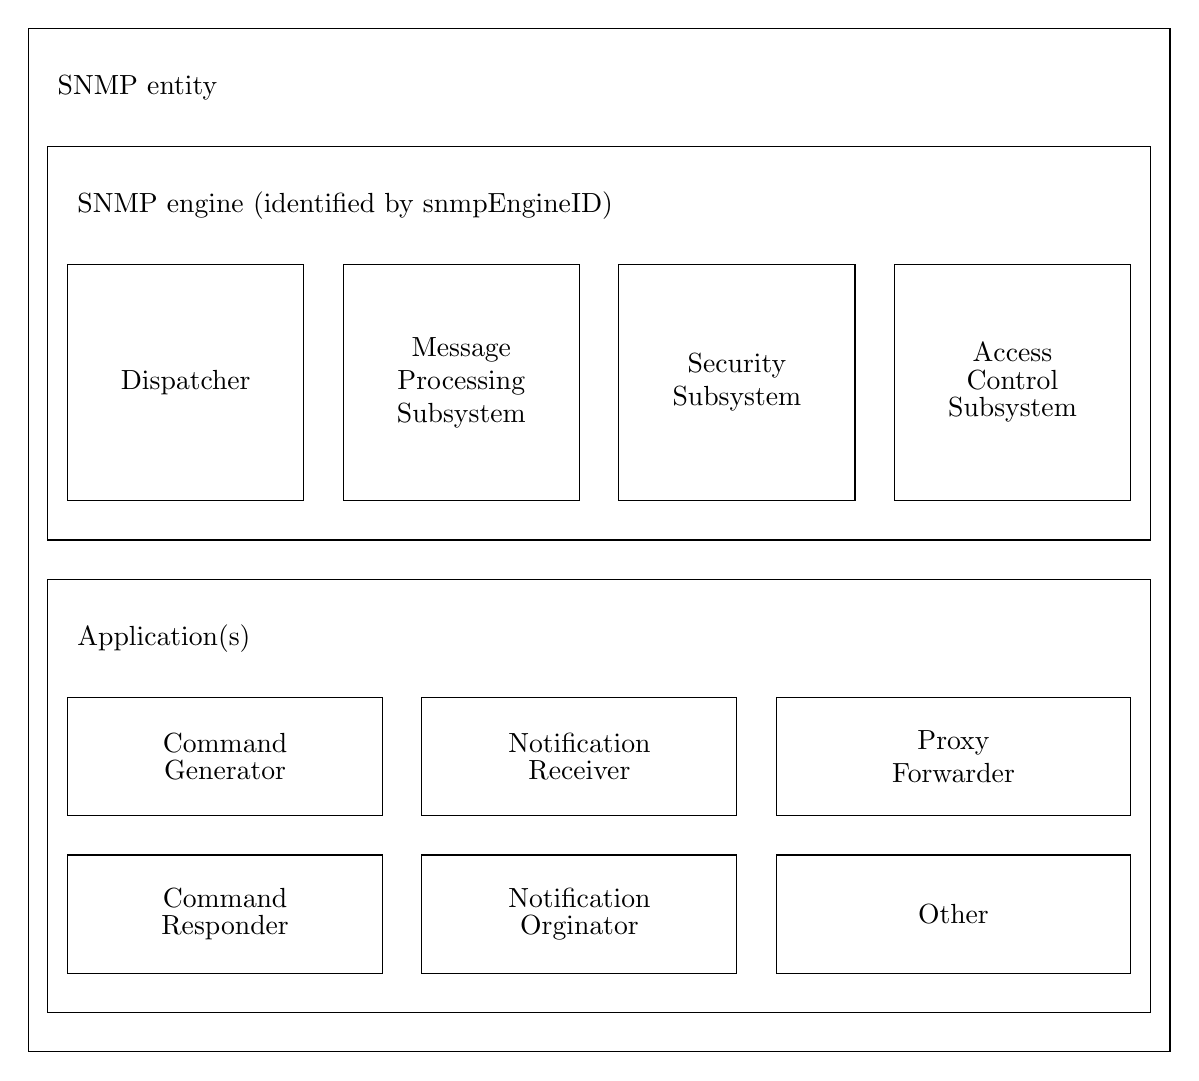
\begin{tikzpicture}
    \tikzstyle{rect} = [shape=rectangle, draw, align=center]

    \draw (0,    0) rectangle (14.5, -13) node[right] at(0.25, -0.75){SNMP entity};

        \draw (0.25, -1.5) rectangle (14.25, -6.5) node[right] at(0.5, -2.25){SNMP engine (identified by snmpEngineID)};

            \draw (0.5, -3)   rectangle (3.5, -6) node[pos=.5] {\shortstack{Dispatcher}};
            \draw (4,   -3)   rectangle (7,   -6) node[pos=.5] {\shortstack{Message\\Processing\\Subsystem}};
            \draw (7.5, -3)   rectangle (10.5,-6) node[pos=.5] {\shortstack{Security\\Subsystem}};
            \draw (11,  -3)   rectangle (14,  -6) node[pos=.5] {\shortstack{Access\\Control\\Subsystem}};

        \draw (0.25, -7) rectangle (14.25,  -12.5) node[right] at(0.5, -7.75){Application(s)};

            \draw (0.5, -8.5) rectangle (4.5, -10) node[pos=.5] {\shortstack{Command\\Generator}};
            \draw (5,   -8.5) rectangle (9,   -10) node[pos=.5] {\shortstack{Notification\\Receiver}};
            \draw (9.5, -8.5) rectangle (14,  -10) node[pos=.5] {\shortstack{Proxy\\Forwarder}};

            \draw (0.5, -10.5) rectangle (4.5,-12) node[pos=.5] {\shortstack{Command\\Responder}};
            \draw (5,   -10.5) rectangle (9,  -12) node[pos=.5] {\shortstack{Notification\\Orginator}};
            \draw (9.5, -10.5) rectangle (14, -12) node[pos=.5] {\shortstack{Other}};
\end{tikzpicture}
\caption{Naming and hierarchy of single elements from a SNMP entity (Adapted from \cite{RFC:RFC3411:2002})}
\label{Figure:SNMP-EntityNaming}
\end{figure}

The purpose of the SNMP engine is to provide services to send, receive, authenticate and encrypt messages, while also handling the access control to managed objects. For these tasks, it contains a Dispatcher, a Message Processing Subsystem, a Security Subsystem, and an Access Control Subsystem. Only one SNMP engine exists per SNMP entity. An overview of the subsystems, their naming, and hierarchy can be found in Figure \ref{Figure:SNMP-EntityNaming}.

Every SNMP engine is identified by a snmpEngineID. This identifier must be unique within an administrative domain. Because only one SNMP engine exists per SNMP entity, this identifier can also be used to identify the SNMP entity.

\newpage
The Dispatcher is used to send and receive SNMP messages. Therefore, it must be able to determine the SNMP version of a message. It provides an abstract interface for the SNMP application to send and receive messages over the network. Only one Dispatcher can exist per SNMP engine.

An SNMP engine also contains one Message Processing Subsystem, which is responsible for preparing messages for sending and extracting data from received messages. One Message Processing Subsystem can contain multiple Message Processing Models (eg. SNMPv3, SNMPv2c, SNMPv1), whereby model processes its matching SNMP message.

The Security Subsystems is part of the SNMP engine and provides services like authentication and privacy. The subsystem may contain one or more models. Only one Security Subsystem can exist per SNMP engine.

Lastly, another subsystem included in an SNMP engine is the Access Control Subsystem, which provides one or more Access Control Models. The default Access Control Model is View-Based. Only one of these subsystems can exist per SNMP engine.

Figure \ref{Figure:SNMP-Manager} shows a typical setup of an SNMP Manager. It has one or more command generators and notification receivers. An instruction is generated in a command generator application and the instruction is sent to the Dispatcher. In the Dispatcher the instruction is encapsulated in a PDU. After that, the Message Dispatcher transfers the data to the Message Processing Subsystem, where the correct SNMP version and its properties are appended. The Message Processing System transfers the message to the Security Subsystem, where security-related information is added. In the next step, the message is passed to the Transport Mapping. This step adds transport-related and transport-protocol-related information to the message. After that, the message is embedded into the Transport Protocol and is delivered over the network. Receiving a message and parsing it works in reverse order. The only difference is that a notification receiver application is receiving the message instead of a command generator application. For further information see Section 4.6.1 in RFC 3411 on page 38 \cite{RFC:RFC3411:2002}.

Figure \ref{Figure:SNMP-Agent} shows a typical setup of an SNMP Agent, which has one or more command receiver applications and notification originator applications. The process of receiving and decoding a message is the same as for an SNMP manager. After the message is decoded, it can be sent to a proxy forwarder application, which is forwarding the message to another SNMP entity, or to the notification originator application and command responder application. These applications may check if the sender is authorized to receive or write the content of the requested MIB entry. They can check if the access is granted by communicating with the access control unit. If access is granted, the content of the MIB entry may be sent back to the origin of the request in reverse order of receiving the message. For further information see Section 4.6.2 in RFC 3411 on page 39 \cite{RFC:RFC3411:2002}.

The snmpEngineID only describes the SNMP engine and the SNMP entities. Because of that, every context (instance of MIB Objects) also needs to be uniquely identified. Every context has a readable name (e.g.: bridge0, bridge1), and additionally, the contextID is provided. If the contextID is the same as the snmpEngineID, the context is only valid on this SNMP entity. If the context is valid over multiple SNMP entities, another contextID may be used, but the combination of contextName and contextID must be unique in the administrative domain. It is also possible that multiple combinations of contextID and contextName exist to identify the same object.

With SNMPv3 three levels of security have been introduced:

\begin{minipage}{\textwidth}
\begin{itemize}
    \item noAuthNoPriv - without authentication and without privacy
    \item authNoPriv - with authentication and without privacy
    \item authPriv - with authentication and with privacy
\end{itemize}
\end{minipage}

\newpage
The security levels are sorted like this: noAuthNoPriv < AuthNoPriv < AuthPriv. Every message has an associated security level and all subsystems and applications are required to provide a value of security level or to hold the same security level while processing data.

\begin{figure}[!h]
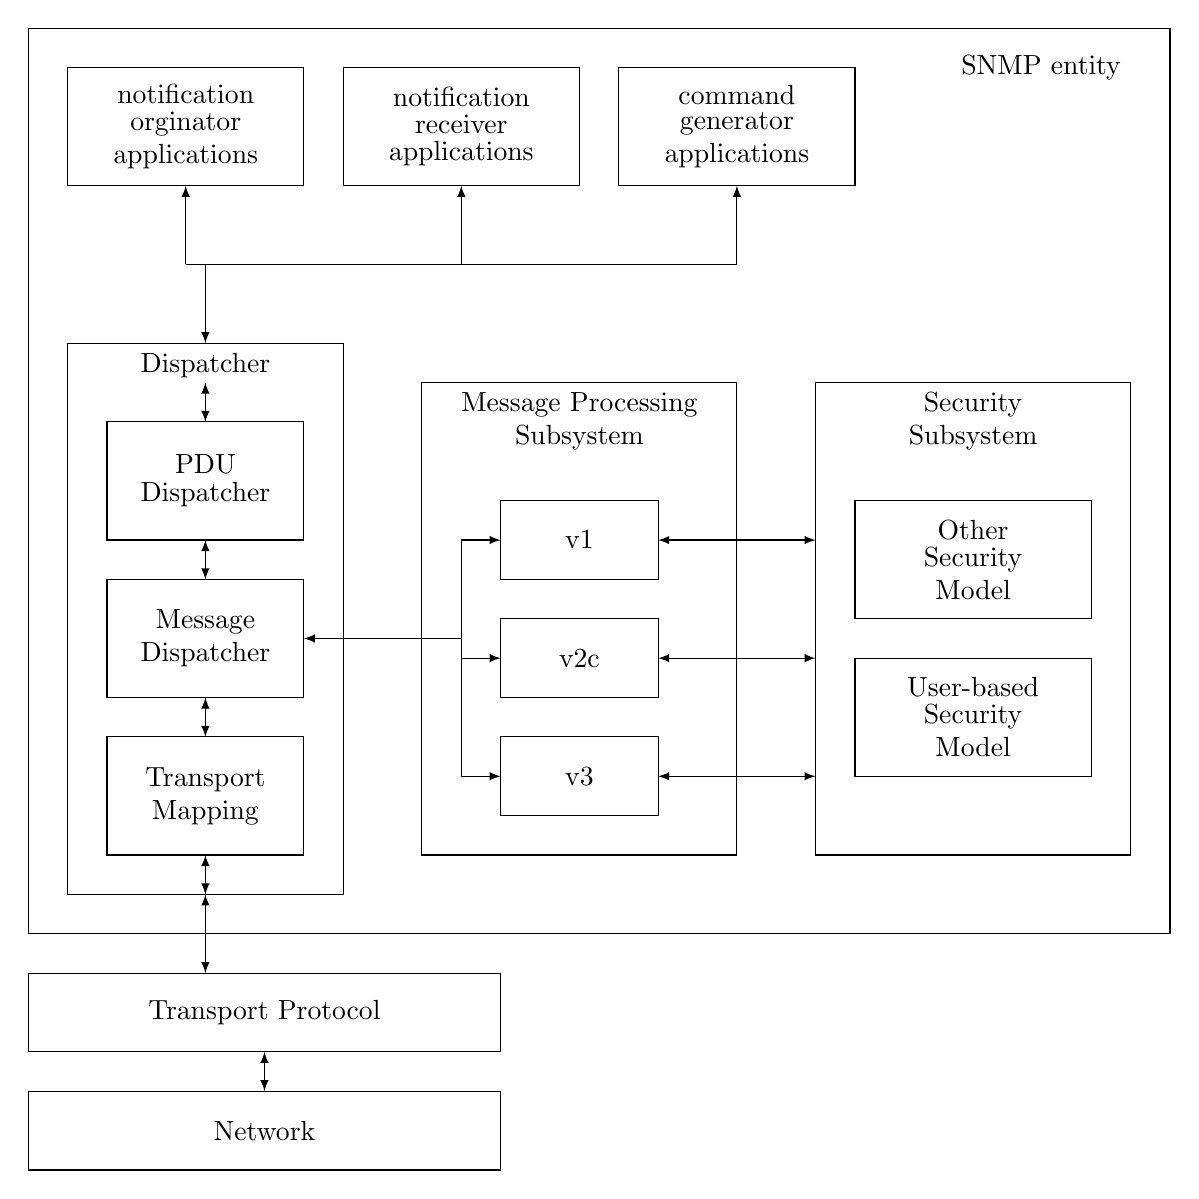
\begin{tikzpicture}
    \tikzstyle{rect} = [shape=rectangle, draw, align=center]

    \draw (0, 0) rectangle (14.5, -11.5)
        node[left] at(14, -0.5) {\shortstack{SNMP entity}};

        \draw (0.5, -0.5) rectangle ( 3.5, -2)
            node[pos=.5] {\shortstack{notification\\orginator\\applications}};
        \draw (4.0, -0.5) rectangle ( 7.0, -2)
            node[pos=.5] {\shortstack{notification\\receiver\\applications}};
        \draw (7.5, -0.5) rectangle (10.5, -2)
            node[pos=.5] {\shortstack{command\\generator\\applications}};

        \draw[latex-]   (2.0, -2) -- (2.0, -3.0);
        \draw[latex-]   (5.5, -2) -- (5.5, -3.0);
        \draw[latex-]   (9.0, -2) -- (9.0, -3.0);
        \draw[-]        (2.0, -3) -- (9.0, -3.0);
        \draw[-latex]   (2.25,-3) -- (2.25,-4.0);

        \draw (0.50, -4) rectangle (4.0, -11)
            node[below] at(2.25,-4) {\shortstack{Dispatcher}};

            \draw (1, -5) rectangle (3.5, -6.5)
                node[pos=.5] {\shortstack{PDU\\Dispatcher}};
            \draw (1, -7) rectangle (3.5, -8.5)
                node[pos=.5] {\shortstack{Message\\Dispatcher}};
            \draw (1, -9) rectangle (3.5, -10.5)
                node[pos=.5] {\shortstack{Transport\\Mapping}};

            \draw[latex-latex]  (2.25, -4.5)  -- (2.25, -5);
            \draw[latex-latex]  (2.25, -6.5)  -- (2.25, -7);
            \draw[latex-latex]  (2.25, -8.5)  -- (2.25, -9);
            \draw[latex-latex]  (2.25, -10.5) -- (2.25, -11);

        
        \draw[latex-]   (3.50, -7.75) -- (5.50, -7.75);
        \draw[-]        (5.50, -6.50) -- (5.50, -9.50);
        \draw[-latex]   (5.50, -6.50) -- (6.00, -6.50);
        \draw[-latex]   (5.50, -8.00) -- (6.00, -8.00);
        \draw[-latex]   (5.50, -9.50) -- (6.00, -9.50);


        \draw (5.00, -4.5) rectangle (9.0, -10.5)
            node[below] at(7.00, -4.5) {\shortstack{Message Processing\\Subsystem}};

            \draw (6, -6.0) rectangle (8, -7.0)
                node[pos=.5] {\shortstack{v1}};
            \draw (6, -7.5) rectangle (8, -8.5)
                node[pos=.5] {\shortstack{v2c}};
            \draw (6, -9.0) rectangle (8, -10.0)
                node[pos=.5] {\shortstack{v3}};

        \draw[latex-latex]   (8, -6.50) -- (10, -6.50);
        \draw[latex-latex]   (8, -8.00) -- (10, -8.00);
        \draw[latex-latex]   (8, -9.50) -- (10, -9.50);
        
        \draw (10.0, -4.5) rectangle (14, -10.5)
            node[below] at(12.0, -4.5) {\shortstack{Security\\Subsystem}};

            \draw (10.5, -6.0) rectangle (13.5, -7.5)
                node[pos=.5] {\shortstack{Other\\Security\\Model}};
            \draw (10.5, -8.0) rectangle (13.5, -9.5)
                node[pos=.5] {\shortstack{User-based\\Security\\Model}};

        \draw[latex-latex]  (2.25, -11)  -- (2.25, -12);

        \draw (0, -12) rectangle (6, -13)
            node[pos=.5] {\shortstack{Transport Protocol}};

        \draw[latex-latex]  (3, -13)  -- (3, -13.5);
        
        \draw (0, -13.5) rectangle (6, -14.5)
            node[pos=.5] {\shortstack{Network}};

\end{tikzpicture}
\caption{Typical structure of an SNMP manager (Adapted from \cite{RFC:RFC3411:2002})}
\label{Figure:SNMP-Manager}
\end{figure}

\begin{figure}[!h]
    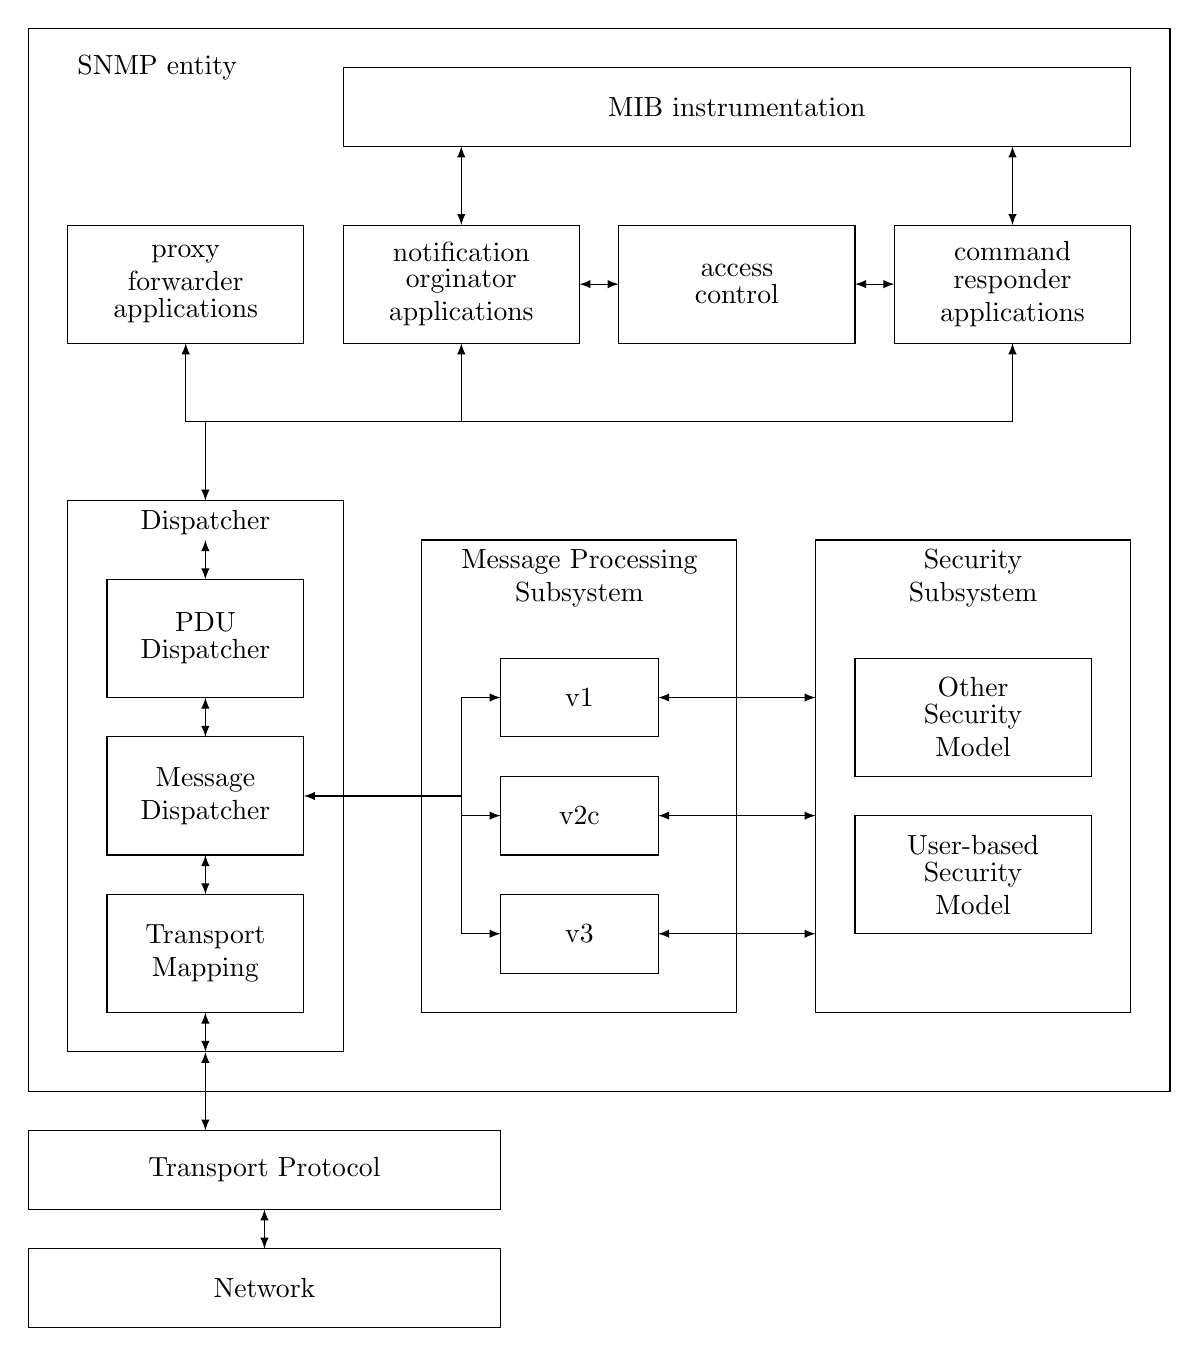
\begin{tikzpicture}
        \tikzstyle{rect} = [shape=rectangle, draw, align=center]
    
        \draw (0, 2) rectangle (14.5, -11.5)
            node[right] at(0.5, 1.5) {\shortstack{SNMP entity}};
    
            \draw (4, 1.5) rectangle (14, 0.5)
                node[pos=.5] {\shortstack{MIB instrumentation}};
    
            \draw[latex-latex]   (5.5, 0.5) -- (5.5, -0.5);
            \draw[latex-latex]   (12.5,0.5) -- (12.5,-0.5);
    
            \draw (0.5, -0.5) rectangle ( 3.5, -2)
                node[pos=.5] {\shortstack{proxy\\forwarder\\applications}};
            \draw (4.0, -0.5) rectangle ( 7.0, -2)
                node[pos=.5] {\shortstack{notification\\orginator\\applications}};
            \draw (7.5, -0.5) rectangle (10.5, -2)
                node[pos=.5] {\shortstack{access\\control}};
            \draw (11,  -0.5) rectangle (14, -2)
                node[pos=.5] {\shortstack{command\\responder\\applications}};
    
            \draw[latex-latex]   (10.5, -1.25) -- (11,  -1.25);
            \draw[latex-latex]   (7.0,  -1.25) -- (7.5, -1.25);
    
            \draw[latex-]   (2.0, -2) -- (2.0, -3.0);
            \draw[latex-]   (5.5, -2) -- (5.5, -3.0);
            \draw[latex-]   (12.5,-2) -- (12.5,-3.0);
            \draw[-]        (2.0, -3) -- (12.5,-3.0);
            \draw[-latex]   (2.25,-3) -- (2.25,-4.0);
    
            \draw (0.50, -4) rectangle (4.0, -11)
                node[below] at(2.25,-4) {\shortstack{Dispatcher}};
    
                \draw (1, -5) rectangle (3.5, -6.5)
                    node[pos=.5] {\shortstack{PDU\\Dispatcher}};
                \draw (1, -7) rectangle (3.5, -8.5)
                    node[pos=.5] {\shortstack{Message\\Dispatcher}};
                \draw (1, -9) rectangle (3.5, -10.5)
                    node[pos=.5] {\shortstack{Transport\\Mapping}};
    
                \draw[latex-latex]  (2.25, -4.5)  -- (2.25, -5);
                \draw[latex-latex]  (2.25, -6.5)  -- (2.25, -7);
                \draw[latex-latex]  (2.25, -8.5)  -- (2.25, -9);
                \draw[latex-latex]  (2.25, -10.5) -- (2.25, -11);
            
            \draw[latex-]   (3.50, -7.75) -- (5.50, -7.75);
            \draw[-]        (5.50, -6.50) -- (5.50, -9.50);
            \draw[-latex]   (5.50, -6.50) -- (6.00, -6.50);
            \draw[-latex]   (5.50, -8.00) -- (6.00, -8.00);
            \draw[-latex]   (5.50, -9.50) -- (6.00, -9.50);
    
    
            \draw (5.00, -4.5) rectangle (9.0, -10.5)
                node[below] at(7.00, -4.5) {\shortstack{Message Processing\\Subsystem}};
    
                \draw (6, -6.0) rectangle (8, -7.0)
                    node[pos=.5] {\shortstack{v1}};
                \draw (6, -7.5) rectangle (8, -8.5)
                    node[pos=.5] {\shortstack{v2c}};
                \draw (6, -9.0) rectangle (8, -10.0)
                    node[pos=.5] {\shortstack{v3}};
    
            \draw[latex-latex]   (8, -6.50) -- (10, -6.50);
            \draw[latex-latex]   (8, -8.00) -- (10, -8.00);
            \draw[latex-latex]   (8, -9.50) -- (10, -9.50);
            
            \draw (10.0, -4.5) rectangle (14, -10.5)
                node[below] at(12.0, -4.5) {\shortstack{Security\\Subsystem}};
    
                \draw (10.5, -6.0) rectangle (13.5, -7.5)
                    node[pos=.5] {\shortstack{Other\\Security\\Model}};
                \draw (10.5, -8.0) rectangle (13.5, -9.5)
                    node[pos=.5] {\shortstack{User-based\\Security\\Model}};
    
            \draw[latex-latex]  (2.25, -11)  -- (2.25, -12);
    
            \draw (0, -12) rectangle (6, -13)
                node[pos=.5] {\shortstack{Transport Protocol}};
    
            \draw[latex-latex]  (3, -13)  -- (3, -13.5);
            
            \draw (0, -13.5) rectangle (6, -14.5)
                node[pos=.5] {\shortstack{Network}};
    
    \end{tikzpicture}
    \caption{Typical structure of a SNMP agent (Adapted from \cite{RFC:RFC3411:2002})}
    \label{Figure:SNMP-Agent}
    \end{figure}

\newpage
~\newpage

\subsection{Protocol}
\label{Section:SNMP-Protocol}
The basic functions of the protocol are defined in RFC3416 \cite{RFC:RFC3416:2002}. It is defined that it should be possible to retransmit a request. Under normal circumstances, the receiver is required to send a response to the originator of the message. If no response is received, the originator can decide if the message should be retransmitted, but the application needs to act responsibly with the retransmission frequency and duration.

The message size is limited to the capabilities of all SNMP entities that are part of the communication. The maximum size of a message is defined by the smallest value of the maximum size that both the receiving SNMP entity can accept and the sending SNMP entity can generate. The maximum size an entity can receive may be known. Otherwise the size is defined by the transport domain when sending the message. The maximum size an entity can generate is defined by local constraints. Each transport mapping defines a minimum size, which every entity needs to be able to consume and produce.

The goal of the GetBulkRequest-PDU is to reduce the number of messages. Therefore, messages should be as large as possible. To achieve this, the PDU is embedding the limits of supported message sizes from the command responder and command generator into the request. It can happen that the maximum message size is bigger than the MTU of the network, leading to fragmentation of the message. Message fragmentation can decrease the reliability of the transfer.

SNMP only requires an unreliable datagram. The protocol encourages the use of UDP to send messages, but other transport mappings can also be used.

PDUs contain a request-id field. The request-id is generated by the sending SNMP entity and added to the Request-PDU. If a response for that request is sent by the receiving entity, the request-id from the received request is used. This makes it easy to match sent requests with the incoming response.  To calculate round-trip time, the request-id needs to be changed if the PDU is retransmitted. A non-zero value of the error-status field in the Response-PDU indicates that an error occurred. The error-index field represents which variable-binding caused the error. Thereby, the error-index is the same as the index of the variable-binding in a variable-binding list.

The different PDUs can contain fields that are not relevant for the specific PDU type. These fields are ignored while processing the PDU by the receiving entity. Every field, even the ignored ones, must have a valid ASN.1(\ref{Section:MIB-Syntax}) syntax and encoding. There can be as many variable bindings as fit into the message size limit, but no more than 21474483647.

\newpage
The GetRequest-PDU is generated and is transmitted by the request of an application. Each variable binding in the variable-binding list is getting processed by the receiving SNMP entity. Every field of the Response-PDU has the same value as the corresponding sent PDU. They are processed as follows: If the variable name exactly matches the name of the accessible variable, then the variable field is set to the value of the accessible variable.  If the name does not match exactly and does not have an OID prefix that matches the requested OID prefix, the value is set to "noSuchObject". Otherwise, the variable field is set to "noSuchInstance".

If any other error occurs, the Response-PDU is set to the same value as the received fields and the error-status field is set to "genError". Else, the error-status field is set to "noError" and the error-index field is set to zero. If the message is shorter than or equals the maximum message size, the Response-PDU is transmitted to the originator. Otherwise, an alternative Response-PDU is generated, with the same values as the received PDU, the error-status field set to "tooBig" and the error-index field set to 0. If this alternate Response-PDU is bigger than the maximal message size, the message is dropped and the snmpSilentDrops counter is increased.

The GetNextRequest-PDU is generated and is transmitted by the request of an application. The variables are processed as follows: The successor variable of the lexicographically order variable names is located. The found name and the value are set in the Response-PDU to the same index as the variable of the GetNextRequest-PDU. If the requested variable has no successor, then the value is set to "endOfMibView" and the name is set to the name of the variable from the GetNextRequest-PDU. The errors are handled in the same way as for the GetRequest-PDU.

The GetBulkRequest-PDU is generated and transmitted by the request of an application. The purpose of this PDU is to request a large amount of data, but it also can be used to retrieve large tables rapidly and efficiently. Every variable is processed on receive and a Responds-PDU is produced with the request-id, but the variables are not mapped one-to-one like in the GetRequest-PDU, GetNextRequest-PDU, and SetRequest-PDU. This PDU has a non-repeaters and max-repetitions field, which is not included in other PDUs. The non-repeaters field contains the number of variables in the variable list where a single-lexicographic successor can be returned, while the max-repetitions field contains the number of lexicographic successors for the remaining variables.

In the following description, we define these variables: $N$ is the value of the non-repeaters field, $M$ is the value of the max-repetitions field, and $R$ is the maximum of variables minus the value of non-repeater fields $N$. The variables get requested as follows: One variable of the Respond is assigned to the first $N$ variables, $M$ variables are requested for the $R$ variables. This results in a total number of $N + (M * R)$ requests. A more detailed explanation is given in RFC 3416 Section 4.2.3 on page 15 \cite{RFC:RFC3416:2002}. The errors are handled the same as for the GetRequest-PDU.

\newpage
The SetRequest-PDU is generated and is transmitted by the request of an application. The receiving entity parses the PDU and produces a response PDU. In the first step, the variables are validated, and if all validations succeed, the variables get altered. These validations are performed:

\begin{itemize}
    \item Access for the variable name is validated. If no access is granted, the error-status is "noAccess".
    \item If the OID prefix does not match any variable that can be created or modified, the error-status is set to "notWriteable".
    \item If the ASN.1 type is inconsistent with the required type, the error-status is set to "wrongType"
    \item If the required length is inconsistent, the error-status is set to "wrongLength"
    \item If the encoding does not match ASN.1, the error-status is set to "wrongEncoding"
    \item If a value is specified that can not be set, the error-status is set to "wrongValue".
    \item If a specified variable does not exist or can not be created, the error-status is set to "noCreation".
    \item If a specified variable does not exist and can not be created under circumstances, the error-status is set to "inconsistentName".
    \item If a variable is specified that can not be created or modified, no matter of the new value, the error-status is set to "notWriteable".
    \item If a value can not be set or modified, but could be under circumstances, the error-status is set to "inconsistentValue".
    \item If the variable needs allocation of a resource that is not available, the error-status is set to "resourceUnavailable".
    \item If the processing fails for another reason, the error-status is set to "genErr".
\end{itemize}

If a requested variable does not exist, it is created and the value is assigned to it. When the same variable should be set multiple times with different values in one request, the behavior is implementation-specific. If an assignment fails, all other assignments from the same request get reverted and the error-status is set to "commitFailed". If it is not possible to revert all assignments, the error-status is set to "undoFailed". It is recommended for implementations to avoid both cases.

\newpage
The SNMPv2-Trap-PDU is generated and is transmitted on behalf of a notification originator application. These PDUs are often used to inform remote entities about events that occurred. The PDUs are not getting confirmed and the destinations for these PDUs are implementation-dependent. The first variables in an SNMPv2-Trap-PDU are sysUpTime.0 and snmpTrapOID.

The InformRequest-PDU is generated and is transmitted on behalf of a notification originator application. Like SNMPv2-Trap, it informs about an event without guarantee of delivery, but adds confirmation. The destination to which it is sent is defined by the notification originator. The first two variables in the PDU are sysUpTime.0 and snmpTrapOID. If an InformRequest-PDU is received, the entity validates the received PDU. If the validation succeeds, the entity presents its content to the appropriate application, generates a Respond-PDU to confirm the PDU, and transmits it.

\subsection{Transport Subsystem}
\label{Section:SNMP-TransportSubsystem}

The goal of the Transport Subsystem (\cite{RFC:RFC5590:2009}) is to provide access to lower-layer security mechanisms. This can include authentication of the sender, encryption, data integrity, and timeliness checking. Examples for these techniques are TLC, Simple Authentication and Security Layer (SASL) as well as SSH. Transport Mappings need to use security protocols the way they were designed. Modified usage often implies that the protocol can not deliver the expected security characteristics. They also should not modify the underlying security protocol, which might change it is security characteristics.

Transport Subsystems must meet the following requirements:
\begin{itemize}
    \item They must follow the architectural modularity requirements.
    \item If establishing the connection between two entities for every message is too expensive, sessions can be used.
    \item The security model must use the same or a higher security level than provided by the transport model.
    \item A message processing model might unpack security-specific parameters from incoming messages, before calling a specific security model.
    \item Authentication and Authorization are separated. Authentication is handled by the security model and Authorization by the access control model.
\end{itemize}

A security name is a human-readable value, that describes the used security protocol and is used by SNMP Applications and the Access Control Subsystem. The transport mapping security name is a human-readable value and is used by the transport and security models to identify the used transport security protocol.

\newpage
The security value consists of two values: the requested security level, and the transport security level. The first value represents the minimum security level required for transport models. It can be used to prevent sending messages via sessions that are not secure enough. The second value represents the security level offered by the session. The security model can use this to ensure the minimum security level for incoming messages for a session.

\subsection{Transport Mapping}
\label{Section:SNMP-TransportMapping}

Transport Mappings are used to describe the way how data is transferred between multiple SNMP entities. An SNMP entity can use multiple transport mappings, but every entity should provide access via UDP over IPv4. If an entity supports IPv4 as Transport Mapping, it must also implement UDP over IPv4. The definition for Transport Mappings can be found in RFC 3417 \cite{RFC:RFC3147:2002}.

It should be mentioned that popular Transport Mappings are "SNMP over UDP over IPv4" \cite{RFC:RFC3147:2002}, "SNMP over UDP over IPv6" \cite{RFC:RFC3147:2002} and "SNMP over IEEE 802 Networks (Ethernet)" \cite{RFC:RFC4789:2006}. To be able to communicate with SNMPv1 entities, a proxy is needed \cite{RFC:RFC2576:2000}. 

\section{LLDP - Link Layer Discovery Protocol}
\label{Section:LLDP}
LLDP (Link Layer Discovery Protocol) is an open and vendor-independent Layer 2 (Data Link Layer) Protocol, which is defined in IEEE Std 802.1AB \cite{IEEE:LLDP:2016}. Its purpose is to advertise the identity and capabilities to the connected network neighbors. Each device needs to run an LLDP Agent, which collects the information of the neighbors and publishes its information periodically.

LLDP data are transferred via Ethernet frames, with a specific multicast destination addresses and a specific EtherType. These frames with the specific multicast destination addresses are not forwarded by switches and routers, but other addresses are permitted.

LLDP is a one-way protocol, the agent can receive and transmit information, but does not directly communicate with other agents. Because of that, LLDP allows to separately enable the receive or transmit functionality. The LLDP agent itself does not provide any functionality to process information. Received information is stored in multiple MIB tables and can be read per SNMP (see Section \ref{Section:SNMP}) or other provided interfaces \cite{IEEE:LLDP:2016}. 

\subsection{Communication}
\label{Section:LLDP-Communication}

For communication, Ethernet frames are used. They contain the destination address, the source address, the EtherType, and the LLDP Data Unit (see Table \ref{Table:LLDP-EthernetFrame}). The destination address is a multicast MAC address. It can be a specified and reserved MAC address by IEEE Std 802.1AB \cite{IEEE:LLDP:2016}, but other MAC addresses are also permitted. The Ethernet frame must contain the EtherType "0x88CC". If the Agent supports EtherType encoding, it shall be encoded in the LLDP Data Unit header. The source address must be the MAC Address of the sender or the sender port.

\begin{table}[ht]
    \begin{tabularx}{\linewidth}{|L{9em}|X|L{5em}|L{5em}|}
        \hline
        \rowcolor{lightgray!60} Destination Address & Source Address & EtherType & LLDPDU \\ 
        \hline
        Multicast Address & MAC Address of LLDP Device & 0x88CC & See \ref{Section:LLDP-LLDPDU} \\ 
        \hline
    \end{tabularx}
    \caption{Simplified structure of a Ethernet Frame for LLDP}
    \label{Table:LLDP-EthernetFrame}
\end{table}

\subsubsection{Supported Destinations Addresses}
\label{Section:LLDP-SupportedDestinationsAddresses}

IEEE Std 802.1AB (\cite{IEEE:LLDP:2016}) contains predefined MAC address groups, that allow filtering the proposal of the Ethernet frames by different network components. These network components are Two-Port MAC Relay (also known as cross-connect Ethernet devices), Service Virtual Local Area Network (S-VLAN), Customer Virtual Local Area Network (C-VLAN), and MAC Bridges (Network Switch).

\paragraph{Nearest bridge group (01:80:C2:00:00:0E):} Packages with this destination address are not propagated by Two-Port MAC Relay (TPMR) components, S-VLAN components, C-VLAN components, and MAC Bridges. This means, packages only contain information about devices attached to the same LAN segment as the recipient.

\paragraph{Nearest non-TPMR bridge (01:80:C2:00:00:03):} Frames using this group as destination are not propagated by S-VLAN components, C-VLAN components, and MAC Bridges. But they are propagated by Two-Port MAC Relay (TPMR) components.

\paragraph{Nearest custom bridge (01:80:C2:00:00:00):} LLDPDU sent with this destination address group are not propagated by C-VLAN components and MAC Bridges. But they are propagated by S-VLAN components and Two-Port MAC Relay (TPMR) components.

\paragraph{Custom groups and custom addresses:} Custom groups or individual addresses could be used, but it can happen that the custom address or group is not implemented on the recipient.

Table \ref{Table:LLDP-SupportedMAC} shows the needed implementation for each destination address group and network device category \cite{IEEE:LLDP:2016}.

\begin{table}[ht]
    \begin{tabularx}{\linewidth}{|L{9em}|X|X|X|X|}
        \hline
        \rowcolor{lightgray!60} Address & C-VLAN Bridge & S-VLAN Bridge & TPMR Bridge & End Station \\ 
        \hline 
        Nearest bridge & Mandatory & Mandatory & Mandatory & Mandatory \\ 
        \hline
        Nearest non-TPMR bridge & Mandatory & Mandatory & Not Permitted & Recommended \\ 
        \hline
        Nearest customer bridge & Mandatory & Not Permitted & Not Permitted & Recommended \\ 
        \hline
        Any other group MAC address & Permitted & Permitted & Permitted & Permitted \\ 
        \hline 
        Any individual MAC address & Permitted & Permitted & Permitted & Permitted \\ 
        \hline 
    \end{tabularx}
    \caption{Support for MAC addresses (Adaption based on \cite{IEEE:LLDP:2016})}
    \label{Table:LLDP-SupportedMAC}
\end{table}

\subsection{LLDP Data Unit (LLDPDU)}
\label{Section:LLDP-LLDPDU}
The LLDP Data Unit contains a sequence of TLVs (see Section \ref{Section:LLDP-TLV}). These contain the information sent by the Agents. The Data Unit frame contains three mandatory TLVs and can contain multiple optional ones.

\begin{table}[ht]
    \begin{tabularx}{\linewidth}{|L{10em}|X|L{6em}|}
    \hline
    \rowcolor{lightgray!60}\textbf{Name}     & \textbf{Description}                                             & \textbf{Requirement} \\
    \hline
    Chassis ID TLV    & An unique identifier from the device sending this package        & Mandatory \\
    \hline
    Port ID TLV       & An identifier for the port the receiving device is connected to. & Mandatory \\
    \hline
    Time to Live TLV  & The time in seconds how long the data can be identified as valid & Mandatory \\
    \hline
    Optional TLV      & See \ref{Section:LLDP-TLV}                                       & Optional  \\
    \hline
    ...               & ...                                                              & ...       \\
    \hline
    Optional TLV      & See \ref{Section:LLDP-TLV}                                      & Optional  \\
    \hline
    End of LLDPDU TLV & Marks the end of a TLV sequence.                                 & Optional \\
    \hline
    \end{tabularx}
    \caption{Structure of a LLDPDU Frame (Adaption based on \cite{IEEE:LLDP:2016})}
    \label{Table:LLDP-LLDPDUFrame}
\end{table}

Every LLDPU needs to contain a number of octets. The octets are starting with 1 and the bits in the octets are numbered from 1 to 8, where 1 is the low-order bit. When bits in an octet are represented as a binary number, the highest bit is the most significant bit. If octets are used to represent a binary number, the lowest octet contains the most significant number. When the LLDPU or parts of it are represented using a diagram, the lowest octet is shown most left of the page and within an octet the highest numbered bit is shown most left \cite{IEEE:LLDP:2016}.

\subsection{Type, Length, Value (TLV)}
\label{Section:LLDP-TLV}
The TLV format represents information and contains its type and length. The first TLV section (see Table \ref{Table:LLDP-TLVStructure}) contains the type of the information and is 7 bits long. The next section includes the length of the information string, it is 9 bits long and represents the total length of the information string in octets. The last section of the TLV contains the information string, which can be 0 to 511 Octets long. The information string can contain binary or alphanumeric data. For encoding alpha-numeric data ,UTF-8 \cite{RFC:RFC3629:2003} shall be used.

\begin{table}[h]
    \begin{tabularx}{\linewidth}{|L{7em}|X|X|}
        \hline
        \rowcolor{lightgray!60} TLV type & TLV information string length & TLV information string \\ 
        \hline
        7 bits & 9 bits & $0 \leq n \leq 511$ Octets  \\ 
        \hline
    \end{tabularx}
    \caption{Structure of a TLV (Adaption based on \cite{IEEE:LLDP:2016})}
    \label{Table:LLDP-TLVStructure}
\end{table}

TLV types can be grouped into two categories. The first category contains basic information for network management and is required by every LLDP implementation. Each TLV of this category has its type specified. The second category is organizationally specified. Each TLV of this category has the same type, but includes an organizationally unique identifier (OUI) and an organizationally-specific TLV subtype. This category is specified by standard groups like IEEE 802.1 and IEEE 802.3. The different LLDP TLV Types as defined in \cite{IEEE:LLDP:2016} are briefly summarized in the following.

\begin{table}[h]
    \begin{center}
    \begin{tabular}{|l|l|l|l|}
        \hline
        \rowcolor{lightgray!60} type & name & usage & reference \\ 
        \hline
        0 & End Of LDDPDU & Optional & \ref{Section:LLDP-EndOfLLDPDU} \\ 
        \hline
        1 & Chassis ID & Mandatory & \ref{Section:LLDP-ChassisID} \\ 
        \hline
        2 & Port ID & Mandatory & \ref{Section:LLDP-PortID} \\ 
        \hline
        3 & Time to Live & Mandatory & \ref{Section:LLDP-TimeToLive} \\ 
        \hline
        4 & Port Description & Optional & \ref{Section:LLDP-PortDescription} \\ 
        \hline
        5 & System Name & Optional & \ref{Section:LLDP-SystemName} \\ 
        \hline
        6 & System Description & Optional & \ref{Section:LLDP-SystemDescription} \\ 
        \hline
        7 & System Capabilities & Optional & \ref{Section:LLDP-SystemCapabilities} \\ 
        \hline
        8 & Management Address & Optional & \ref{Section:LLDP-ManagementAddress} \\ 
        \hline
        9-126 & Reserved & --- & --- \\ 
        \hline
        127 & Organizationally Specific & Optional & \ref{Section:LLDP-OrganizationallySpecific} \\ 
        \hline
    \end{tabular}
    \caption{The value of all TLV types (Adaption based on \cite{IEEE:LLDP:2016})}
    \label{Table:LLDP-TLVTypes}
    \end{center}
\end{table}

\subsubsection{End Of LLDPDU TLV}
\label{Section:LLDP-EndOfLLDPDU}
\textit{This TLV type is optional and uses type value 0.} It is 2-octets long and contains only zeros, and it is used to mark the end of a TLV sequence in an LLDPDU frame.

\subsubsection{Chassis ID TLV}
\label{Section:LLDP-ChassisID}
\textit{This TLV type is mandatory and uses type value 1.} It is up to 258 octets long and contains an identifier that can be associated with the transmitting agent. It contains an 8-bit subtype at the beginning of the information string because there are several ways to identify an agent. The subtype can classify a chassis component, interface alias, port component, MAC address, network address, interface name, or a locally assigned string. Each LLDPDU shall only contain one Chassis ID TLV and it shall be the first TLV in an LLDPDU frame.

\subsubsection{Port ID TLV}
\label{Section:LLDP-PortID}
\textit{This TLV type is mandatory and uses type value 2.} It is up to 258 octets long and contains an identifier, which can be associated with the port of the transmitting agent. It contains an 8-bit subtype at the beginning of the information string because there are several ways to identify the port of an agent, like the Chassis ID. The subtype can classify an interface alias, port component, MAC address, network address, interface name, agent circuit ID, or a locally assigned string. Each LLDPDU shall only contain one Port ID TLV and it shall be the second TLV in an LLDPDU frame. The port ID shall be constant while the port remains operational.

\subsubsection{Time To Live TLV}
\label{Section:LLDP-TimeToLive}
\textit{This TLV type is mandatory and uses type value 3.} It is 4 octets long and represents the number of seconds that the receiving agent can assume the attached information as valid. If the time to live contains a non-zero value, the receiving agent is notified to replace old saved information with the attached information. If the time to live is set to zero, the receiving agent is notified to delete all information associated with this agent. This may be used to indicate a shutdown of the sending port. Each LLDPDU shall only contain one Time to Live TLV and it shall be the third TLV in an LLDPDU frame.

\subsubsection{Port Description TLV}
\label{Section:LLDP-PortDescription}
\textit{This TLV type is optional and uses type value 4.} It is up to 257 octets long and contains an alpha-numeric string that describes the sending port. If \textit{ifDesc} object \cite{RFC:RFC2863:2000} is implemented, it should be used for this field. Each LLDPDU shall only contain one Port Description TLV.

\subsubsection{System Name TLV}
\label{Section:LLDP-SystemName}
\textit{This TLV type is optional and uses type value 5.} It is up to 257 octets long and contains an alpha-numeric string of the system name from the sender. If \textit{sysName} object \cite{RFC:RFC3418:2002} is implemented, it should be used for this field. Each LLDPDU shall only contain one System Name TLV.

\subsubsection{System Description TLV}
\label{Section:LLDP-SystemDescription}
\textit{This TLV type is optional and uses type value 6.} It is up to 257 octets long and contains an alpha-numeric string of a textual description from the sender. If sysDescr object \cite{RFC:RFC3418:2002} is implemented, it should be used for this field. Each LLDPDU shall only contain one System Description TLV.


\subsubsection{System Capabilities TLV}
\label{Section:LLDP-SystemCapabilities}
\textit{This TLV type is optional and uses type value 7.} It is 6 octets long and contains bit mask of functions the system is capable and functions the system has enabled. A system can have multiple capabilities and multiple can also be enabled. The bitmask fields are two octets long and can represent following capabilities:

\begin{minipage}{\textwidth}
\begin{itemize}
    \item repeater
    \item MAC Bridge component
    \item 802.11 Access Point
    \item router
    \item telephone
    \item DOCSIS cable device
    \item station only
    \item C-VLAN component
    \item S-VLAN component
    \item Two-port MAC Relay
    \item other
\end{itemize}
\end{minipage}

Each LLDPDU shall only contain one System Description TLV.

\subsubsection{Management Address TLV}
\label{Section:LLDP-ManagementAddress}
\textit{This TLV type is optional and uses type value 8.} It is up to 169 octets long and contains the management address of a device to reach higher layer protocols. This TLV type also provides space to include the system interface number and an object identifier (OID), if they are known \cite{IEEE:LLDP:2016}. In Table \ref{Table:LLDP-ManagementAddressTLVStructure} the structure of the information string can be seen.

\begin{table}[h]
    \begin{tabularx}{\linewidth}{|X|X|X|C{4em}|C{4em}|C{3em}|C{3em}|}
        \hline
        \rowcolor{lightgray!60} management address string length & management address subtype & management address & interface number subtype & interface number & OID string length & OID \\ 
        \hline
        1 octet & 1 octet & 1-31 octets & 1 octet & 4 octets & 1 octet & 0-128 octets \\ 
        \hline
    \end{tabularx}
    \caption{Structure of the information string from a Management Address TLV (Adaption based on \cite{IEEE:LLDP:2016})}
    \label{Table:LLDP-ManagementAddressTLVStructure}
\end{table}

The management address subtype contains the type of an address represented in the management address field. It can be one of the types defined in ianaAddressFamilyNumber module \cite{RFC:RFC3232:2002}.

The management address should contain a Layer 3 address. If no management address is available, the field should contain the MAC address of the sender or the MAC address of it is port.

The interface number subtype describes the value of the interface number field. The following values are defined: Unknown, ifIndex, system port number. If the type is Unknown, the interface number field must only contain zeroes.

The object identifier (OID) field contains an identifier of the type of the hardware component or the protocol entity associated with the indicated management address. The OID shall be ASN.1 \cite{ISO:ISO8824-1:2015} encoded. If no OID is provided, this field shall be skipped.

At least one Management Address TLV should be included in every LLDPDU, the address provided should be the address with the best management capabilities. If more than one Management Address TLV is provided, each address shall be different.

\subsubsection{Organizationally Specific TLVs}
\label{Section:LLDP-OrganizationallySpecific}
\textit{This TLV type is optional and uses type value 127.} This TLV type was created to extend the information that can be advertised by an agent. This type can be specified by a standardizing organization, but also by individual software and equipment vendors. The information string contains a three octets long organizational unique identifier (Clause 8 of IEEEStd 802-2014), one-octet long unique organizationally defined subtype, and an up to 507 octets long organizationally defined information string.


\newpage
\section{NETCONF - Network Configuration Protocol}
\label{Section:NETCONF}

The Network Configuration Protocol (NETCONF) was first published in December 2006 as RFC 4741\cite{RFC:RFC4741:2006}. It was created as the successor to SNMP (see Section \ref{Section:SNMP}) to modernize, simplify, and unify network management.  The protocol was updated in June 2011 with RFC 6241\cite{RFC:RFC6241:2011}. The updated version defines the protocol as follows.

NETCONF uses remote procedure calls (RPC) to send and receive data. The data are encoded in XML. For communication between client and server, secure and connection-oriented sessions are used. Administrative devices are called clients, while network devices are called servers. A server can support one or more sessions. Configuration changes can only be done by authorized sessions and the effects of these changes must be visible to all active sessions.

It is possible for the client to discover the capabilities of a server. This helps the client to adapt its behavior to the capabilities of the server. Capabilities can have dependencies on other capabilities and a server must support all depending capabilities to support a capability.

The protocol is separated into four layers:

\begin{minipage}{\textwidth}
\begin{itemize}
    \item Secure Transport (Layer 1) -  The task of this layer is to provide a path between client and server across the network. The path can be provided via any protocol that fulfills the basic requirements.
    \item Messages (Layer 2) - This layer provides a mechanism for encoding RPCs and notifications.
    \item Operations (Layer 3) - Contains a set of base protocol operations.
    \item Content (Layer 4) - Contains data of the device.
\end{itemize}
\end{minipage}

To specify data models, the YANG data model language (\cite{RFC:RFC6020:2010}) was created. It covers the operations and content layer.

Transport protocols need to provide reliable and sequenced data delivery connections and automatically release requested resources on connection close. Moreover, authentication, data integrity, confidentiality, and replay protection must be provided. The protocol is responsible for establishing the connection between server and client. A NETCONF peer assumes that the authentication is handled by the protocol. Every NETCONF implementation must provide and support the SSH mapping (\cite{RFC:RFC6242:2011}).